%%%%%%%%%%%%%%%%%%%%%%%%%%%%%%%%%%%%%%%%%%%%%%%%%%%%%%%%%%%%%%%%%%%%%%%%%%%%%%%%
%2345678901234567890123456789012345678901234567890123456789012345678901234567890
%        1         2         3         4         5         6         7         8

\documentclass[letterpaper, 10 pt, conference]{ieeeconf}  % Comment this line out if you need a4paper

%\documentclass[a4paper, 10pt, conference]{ieeeconf}      % Use this line for a4 paper

\IEEEoverridecommandlockouts                              % This command is only needed if
                                                          % you want to use the \thanks command

\overrideIEEEmargins                                      % Needed to meet printer requirements.

%In case you encounter the following error:
%Error 1010 The PDF file may be corrupt (unable to open PDF file) OR
%Error 1000 An error occurred while parsing a contents stream. Unable to analyze the PDF file.
%This is a known problem with pdfLaTeX conversion filter. The file cannot be opened with acrobat reader
%Please use one of the alternatives below to circumvent this error by uncommenting one or the other
%\pdfobjcompresslevel=0
%\pdfminorversion=4

% See the \addtolength command later in the file to balance the column lengths
% on the last page of the document

% The following packages can be found on http:\\www.ctan.org
\usepackage{graphics} % for pdf, bitmapped graphics files
\usepackage{epsfig} % for postscript graphics files
\usepackage{mathptmx} % assumes new font selection scheme installed
%\usepackage{times} % assumes new font selection scheme installed
\usepackage{amsmath} % assumes amsmath package installed
\usepackage{amssymb}  % assumes amsmath package installed
%\usepackage{algorithmicx}
%\usepackage[Algorithm,ruled]{algorithm}
%\usepackage{algpseudocode}
\usepackage{tabularx}
\usepackage{multirow}
\usepackage{color}
\usepackage{url}
%\usepackage{balance}
\usepackage{subcaption}
\usepackage{breqn}
\usepackage{algorithm2e}
\usepackage{dblfloatfix} 
\usepackage[export]{adjustbox}
\usepackage{tabulary,booktabs}
%\usepackage{verbatim}
%\usepackage{flushend}

\newcommand{\junk}[1]{}
\newcommand{\abs}[1]{\left| #1 \right|} %| |
\newcommand{\comment}[1]{\textcolor{red}{#1}}



\title{\LARGE \bf
COMP0129: Example Overleaf Document
}

\author{Dimitrios Kanoulas$^{1}$% <-this % stops a space
\thanks{$^{1}$Department of Computer Science, University College London, Gower Street, WC1E 6BT, UK. {\tt\small {d.kanoulas}@ucl.ac.uk}}}%

\date{01 January 2021} %it will not be displayed

\begin{document}

\maketitle
\thispagestyle{empty}
\pagestyle{empty}

\begin{abstract}
This is an example template for the Overleaf documentation.
\end{abstract}

\section{INTRODUCTION}\label{Sec:intro}
This is an introduction to $\LaTeX$ for the COMP0219 course.  The basic $\LaTeX$ tricks you may want are the following.  First, make sure that you write all your text in the main.tex.  Whenever you want to check the .pdf file, press the PDF button on the left sidebar and click: Recompile.  Secondly, you should be able to include figures and images in your document, which is done as follows (give always a label):

In Fig.~\ref{Fig:universe} we show a picture of the universe!

\begin{figure}[ht!]
  \centering
  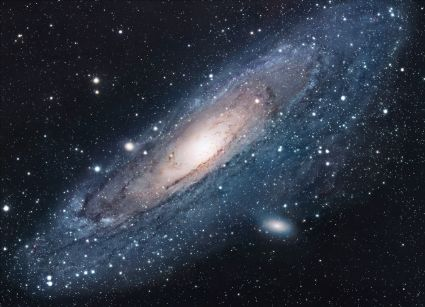
\includegraphics[scale=1.7]{figures/universe.jpg}
  \caption{The Universe}
  \label{Fig:universe}
\end{figure}
\section{METHODOLOGY}\label{Sec:method}
This section introduces the methodology.

\subsection{Sections and subsections}\label{Sec:general}
You can split a section to subsections, and even reference them.  For instance Section~\ref{Sec:intro} is the introduction.  You can also reference the figures.  For instance Fig.~\ref{Fig:universe} is a picture of the universe.  Note that you should upload a figure/picture in the same folder and the main.tex file (using the upload button in the left sidebar).  Also you can add references, which have a special format stored in references.bib file.  To reference a paper you can do in the following way: paper~\cite{Adams1995, Kanoulas2019} talks about the universe.

\subsection{Math}
Math text in $\LaTeX$ are going between dollar signs: $^{0}T_{1}$ is a transformation from frame ${1}$ to frame ${2}$.  The underscore is for subscripts and the hat for superscripts, i.e. $a^2$ and $b_2$.  Also we can include a bit more complex equations in the following way:

\begin{equation}
    ^{0}T_{1} =
    \begin{bmatrix}
    &           & &           \\
    & ^{0}R_{1} & & ^{0}t_{1} \\
    &           & &           \\
    0 & 0 & 0 & 1
    \end{bmatrix}
\end{equation}
\section{CONCLUSIONS AND FUTURE WORK}\label{Sec:concl}
I will keep this document updated when new techniques are needed.  Google is always there for you to find the right way to write in $\LaTeX$, although you can also read any $\LaTeX$ Cheat Sheet, e.g.\\ \url{https://www.nyu.edu/projects/beber/files/Chang_LaTeX_sheet.pdf}


\bibliographystyle{IEEEtran}
\bibliography{references}
\end{document}